\section{\textbf{Introduction}}\label{sec:chap04:intro}
With the pervasive roll out of the \ac{4G} cellular networks, online video streaming in smartphones has become one of the most popular modes of entertainment~\cite{CISCO2019}, especially in many developing countries. The availability of ultra cheap data plans, affordable smartphones, and local language based content on YouTube, Netflix, etc., has led to a record increase in the number of mobile video subscribers as well as their engagement time~\cite{Mobstat_2019}.  Subscribers have  shown an inclination towards watching streaming videos even while travelling, irrespective of the distances travelled. Provisioning the expected \ac{QoE} to video users during travelling requires the reception of a stable connection quality at the \acp{UE}, which often eludes users in developing nations. This is because in these countries service providers often compromise on the network infrastructure to provide low cost internet~\cite{Poor_Inf_2019_2}. \\
\indent Another non-negligible impact of mobility on video streaming in  smartphones is the drainage of battery power.  Video streaming itself is a power hungry application~\cite{Xin2012}. Our experiments show that under mobility, video streaming apps consume even more power (\S\ref{sec:chap04:motivation}). The reason for this can be attributed to the fluctuating connection quality experienced while travelling.  This paper proposes to improve the smartphone battery usage through the design of an energy efficient video streaming algorithm that leverages the fluctuating cellular network throughput to choose optimal bitrates while not compromising on the required \ac{QoE}s. \\
\indent To establish the cellular connectivity scenario, 
we have carried out an extensive measurement-based study for eleven months over five different cities in India, including urban areas as well as while travelling on highways (\S\ref{sec:chap04:motivation}). We have recorded the signal received by  medium budget Moto G5 and Micromax phones, while using the cellular data connection of leading service providers in India, like Airtel, Reliance Jio, and Vodafone.
\begin{figure}[h]
	\captionsetup[subfigure]{width=0.7\linewidth}
	\begin{center}
		\subfloat[\label{fig:chap04:technology_with_traj}Trajectory of a VoLTE-enabled android phone inside an academic campus. Associated network standards (4G, HDPA, UMTS, EDGE) highlighted using different colours)]{
			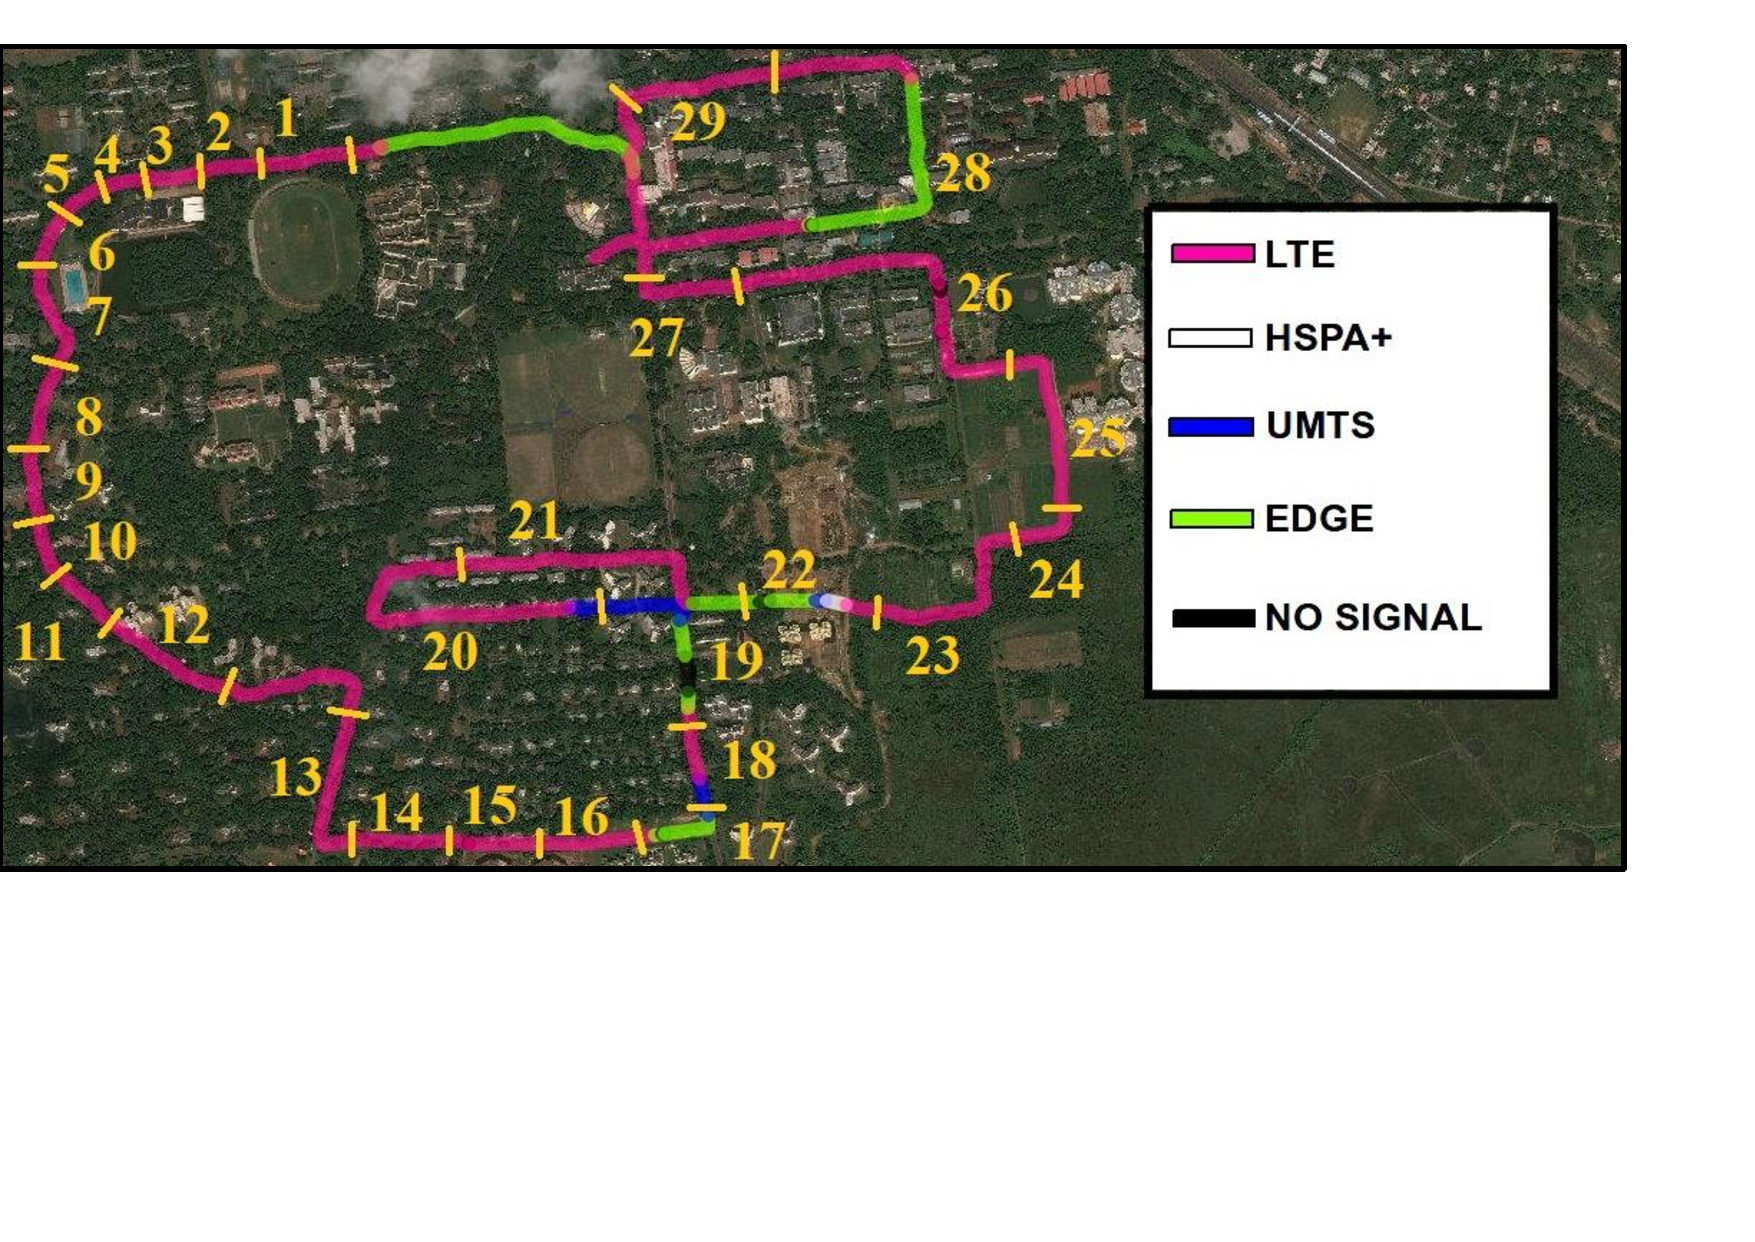
\includegraphics[width = 0.7\linewidth,trim={0cm 6cm 2cm 1cm}]{figures/traj.pdf}
		}\\
	\vspace{+5mm}
		\subfloat[\label{fig:chap04:pcap_RSSI}Packet trace of a 360p Youtube video download with the temporal variation in the \ac{RSSI} during the download]{
			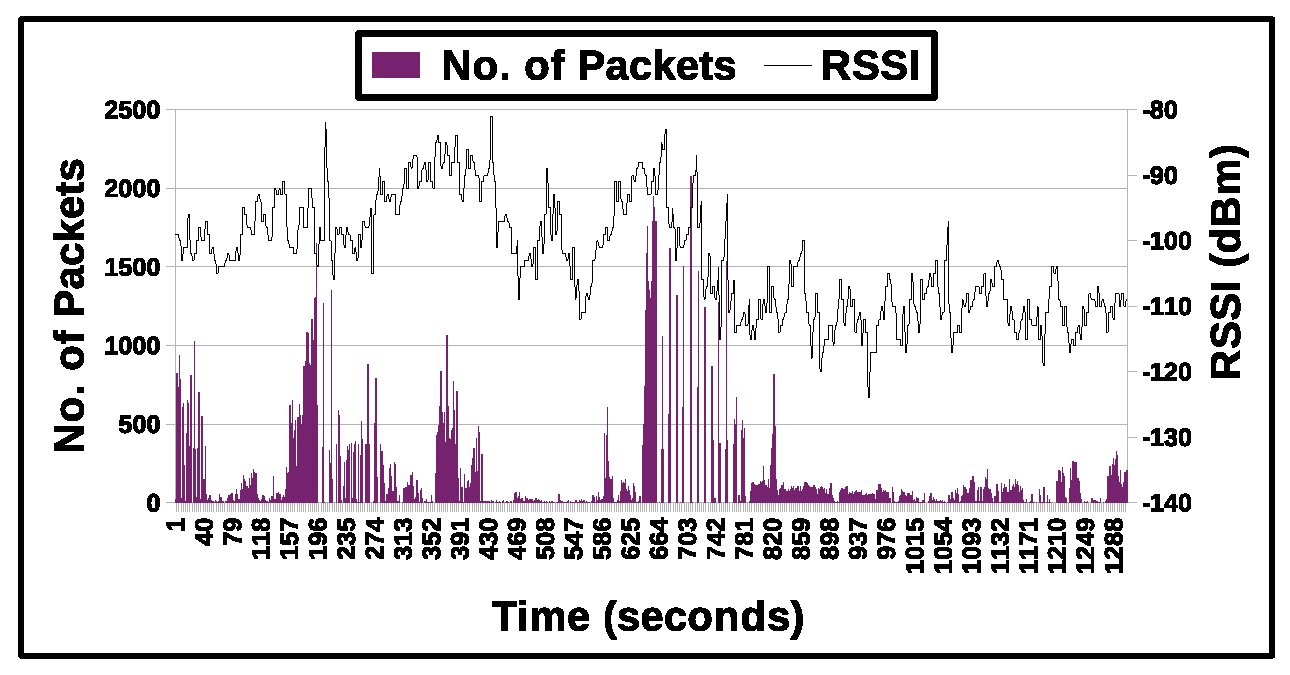
\includegraphics[width=0.7\linewidth,trim={0cm 0cm 0cm 1cm}]{figures/video_rssi_thrpt.eps}
		}
	\end{center}
	\caption{ Experimental Observations}
\end{figure}
%\begin{figure*}[t]%
%\centering
%\subfigure[Trajectory of a VoLTE-enabled android phone inside an academic campus. Associated network standards (4G, HDPA, UMTS, EDGE) highlighted using different colours\vspace*{-0.5cm}]{%
%\label{fig:technology_with_traj}%
%	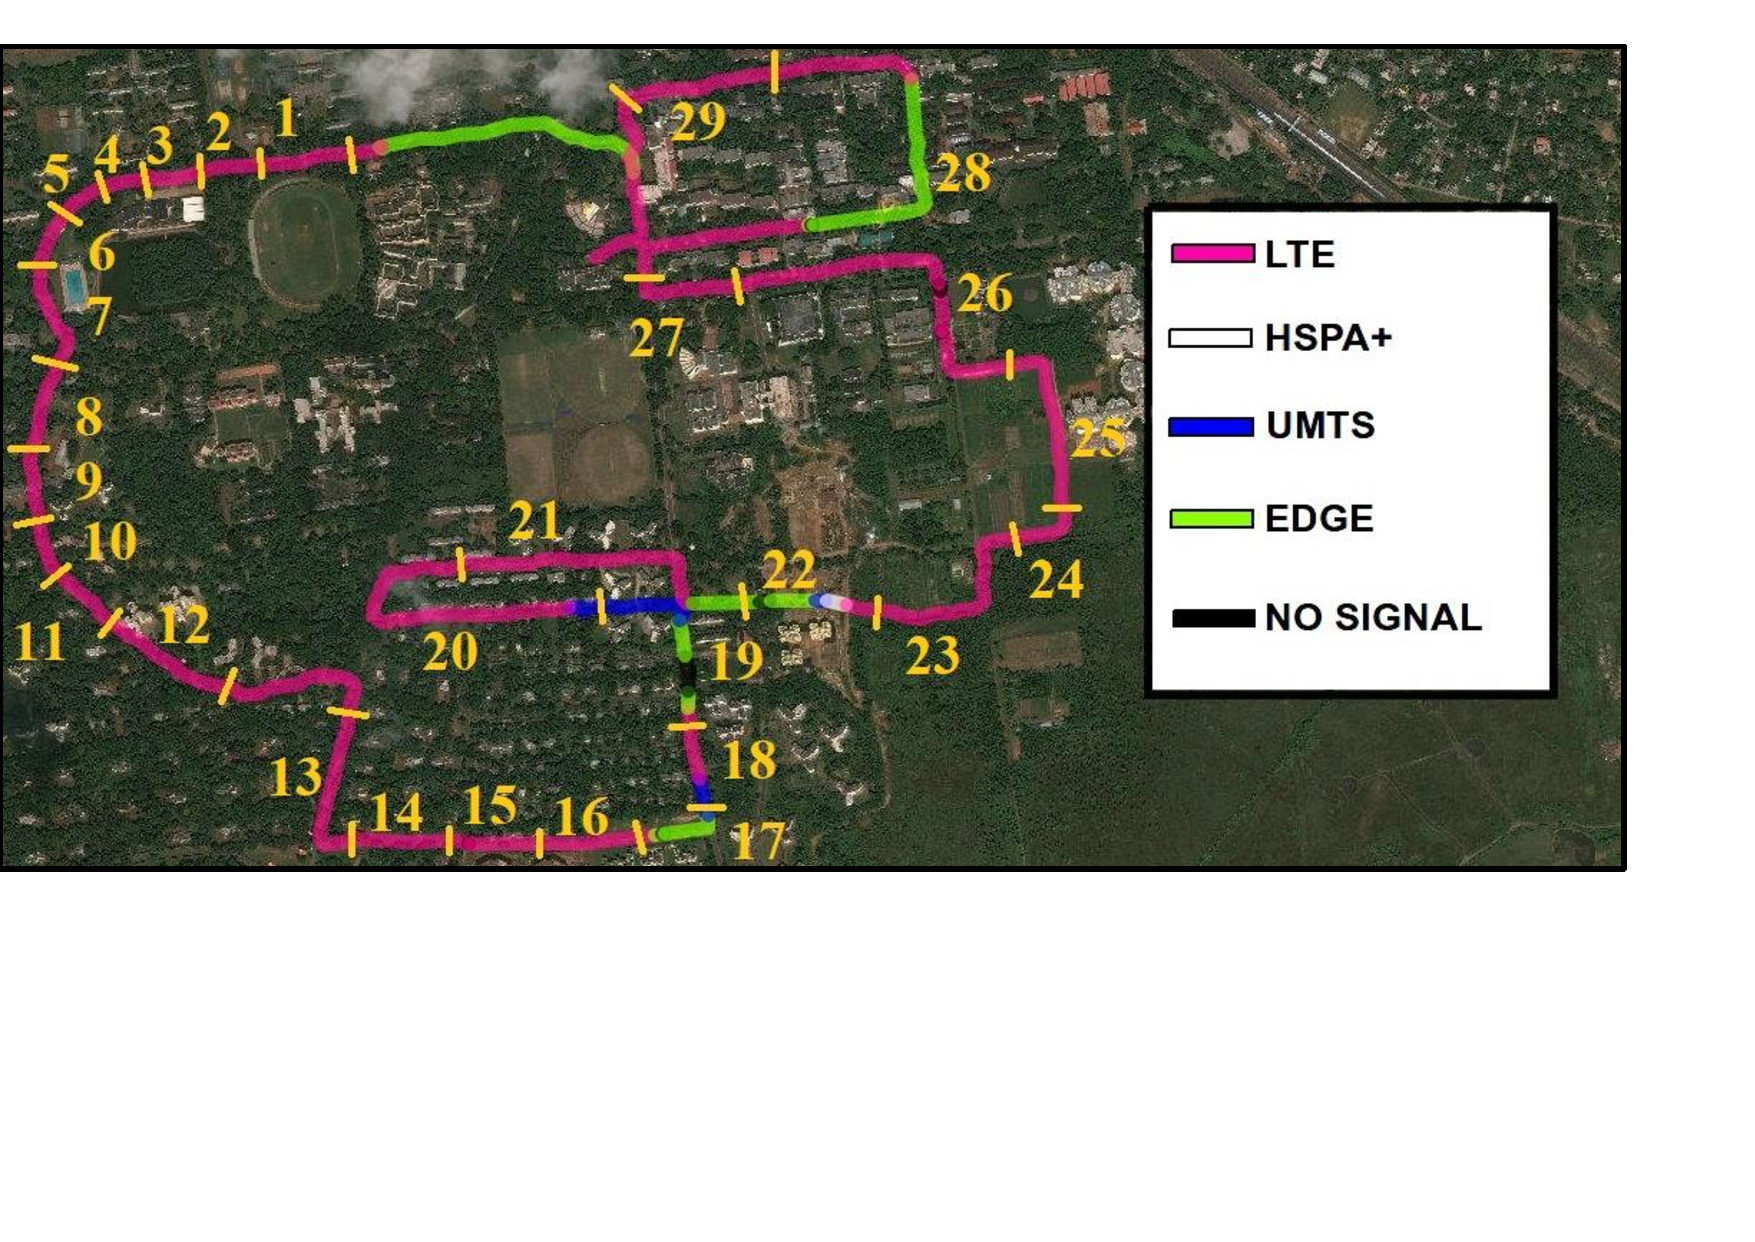
\includegraphics[width = 0.4\textwidth,trim={1cm 7cm 2cm 1cm}]{figures/traj.pdf}}%
%\hspace{2cm}
%\subfigure[Packet trace of a 360p Youtube video download with the temporal variation in the \ac{RSSI} during the download]{%
%\label{fig:pcap_RSSI}%
%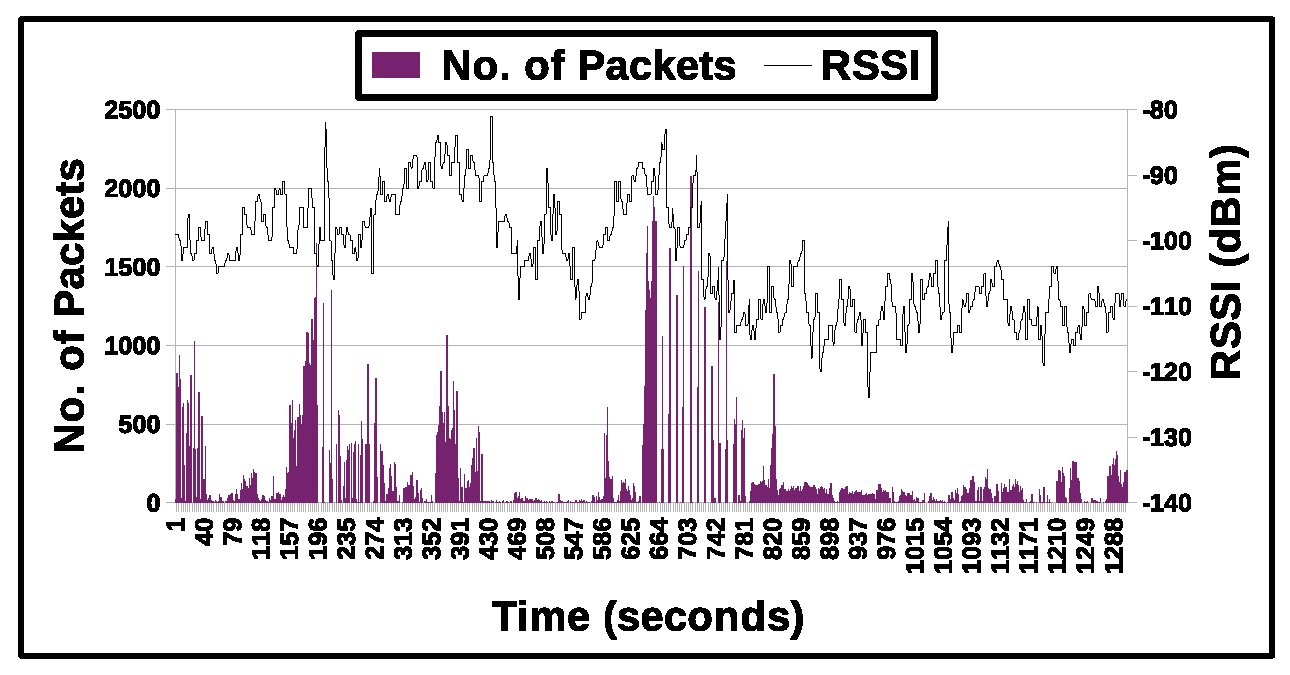
\includegraphics[width=0.4\textwidth,trim={0cm 0cm 0cm 1cm}]{figures/video_rssi_thrpt.eps}}%
%\caption{Experimental Observations}\vspace*{-0.5cm}
%\end{figure*}
A \textit{key finding} of this experiment is shown in Fig.~\ref{fig:chap04:technology_with_traj}, which displays the trajectory of a Moto G5 phone connected to the Airtel network on a single day over the IIT Kharagpur campus area of $8.5$ sq.km. It is seen that even within the small area covered, the phone connects to different generations of cellular technologies, each highlighted in different colours. Two inferences can readily be drawn from Fig. Fig.~\ref{fig:chap04:technology_with_traj}. (i) A service provider does not guarantee a complete \ac{4G} connectivity across the entire coverage region. A \ac{UE} often has to fallback to legacy \ac{3G} or \ac{2G} networks. (ii) Even when connected to \ac{4G}, the signal strength shows random variations. For example, for the experiments conducted, the \ac{RSSI} of \ac{4G} networks fluctuates between $-87$dBm to $-115$dBm. This portrays the typical connectivity scenario in many regions in India.
Another important observation from our experiments, shown in Fig.~\ref{fig:chap04:pcap_RSSI}, is that the volume of data downloaded by video players is not always commensurate with the current network signal strength. Several opportunities to download large chunks of data at high signal strength conditions remain unexploited.


\indent Video streaming applications, including live streaming, predominantly use \ac{DASH} \cite{stockhammer2011dynamic}. In this protocol, the target video is broken into chunks of fixed playback time, and multiple copies of each chunk is stored  at different quality levels, i.e., bitrates.  The client side video player uses \ac{ABR} algorithms~\cite{mao2017neural,Spiteri2016,yin2015control,Raca2019,Akhtar2018}
to decide on the  bitrate at which the next chunk is to be fetched. Existing \ac{DASH} algorithms  primarily take bitrate decisions based on the estimated network throughput or the playback buffer size while attempting to improve user's \ac{QoE}. We, on the other hand, hypothesize that it is possible to significantly lower the energy usage without sacrificing \ac{QoE} if we intelligently utilize the nuances of the cellular network throughput fluctuation during ABR streaming.


\indent To this end, we build an energy
efficient video player {\bf EnDASH} as a wrapper over \ac{DASH} (\S\ref{sec:chap04:sys_overview}).
EnDASH predicts the average cellular network throughput over a finite future time window to take decisions on the opportune fetching of video chunks by dynamically increasing the playback buffer size (\S\ref{sec:chap04:sys_overview}). So, it (i) predicts the the cellular network link throughput from radio related parameters (\S\ref{sec:chap04:thpre}), (ii) then uses the predicted throughput to predict the playback buffer length, and (iii) finally uses the predicted buffer length to choose optimal bitrates for future chunks. Thus, EnDASH consists of three prediction modules, of which the throughput prediction uses random forest learning (step (i)). However, EnDASH works over a smartphone connected to a cellular network which is a randomly varying environment. So, it uses Deep Reinforcement Learning (RL) for the buffer-length prediction mechanism (step (ii)) and bitrate adaptation (step (iii)), which allows EnDASH to exploit the actual performance of previous choices to tune its operation to the current characteristic of the network.  Consequently, EnDASH can start without any apriori knowledge and gradually learn through exploration and exploitation.  The playback buffer length and bitrate decision engines use Deep Neural Networks to map `raw' observations to outputs. These two engines operate using $A3C$ \cite{mao2017neural}, a state-of-the-art actor-critic RL algorithm, and run asynchronously with respect to one another. We train individual prediction modules over a large corpus of collected data traces and evaluate EnDASH using an emulation environment.


\indent Evaluation using our emulation platform shows that in comparison to existing \ac{ABR} algorithms~\cite{mao2017neural,Spiteri2016,yin2015control}, EnDASH significantly improves the energy savings in smartphones (\S\ref{sec:chap04:evaluation}). Energy saved from playing a $2200$ second video using EnDASH can be used to gain an additional $1440$ seconds of video playback time in comparison to the popular Pensieve algorithm~\cite{mao2017neural}. The energy savings, however, comes at the cost of marginally reduced \ac{QoE}.
One of the most salient features of EnDASH, which sets it apart from existing \ac{ABR} algorithms~\cite{mao2017neural,Spiteri2016,Sengupta2018,yin2015control,Raca2019,Akhtar2018,Schulman2010} is that its throughput prediction engine captures the impact of not only the received signal strength but also other network related parameters, such as different technologies and vertical handovers. 
The Mean Absolute Percentage Error (MAPE) of the throughput prediction engine of EnDASH varies from $8\%$ to $13\%$ across different scenarios. The improvement is particularly pronounced in regions having a substantial presence of legacy networks.
The improved throughput prediction assists the EnDASH RL engine to accurately capture the playback buffer evolution, which in turn aids the video segment download in an energy-efficient but QoE favourable manner.\vspace*{-0.2cm}
